% siminos/spatiotemp/chapter/KSspaceInt.tex
% $Author: predrag $ $Date: 2019-09-22 00:02:44 -0400 (Sun, 22 Sep 2019) $

% called by
%           siminos/spatiotemp/chapter/spatiotemp.tex
%           siminos/tiles/GuBuCv17.tex

%\subsection{Temporally periodic \KS}
%\label{sect:KSspaceInt}
%\hfill     2016-02-04 Burak

Consider next the case of temporally periodic velocity field
\beq
    u(\conf, \zeit) = u(\conf, \zeit + \period{})
\label{e-PeriodicBC}
\eeq
on temporal domain of fixed period $\period{}$,
and any \conf, \ie, cylinder $(\conf,t) \in \reals \times [0,\period{})$, see
\reffig{fig:spaceTime1}\,(b).
%\KSe\ in one space dimension is
%\beq
%    u_\zeit =  - u u_\conf
%    -u_{\conf \conf}-u_{\conf \conf \conf \conf}\,,
%    \label{e-ks2}
%\eeq
%where subscripts denote partial derivatives.
In order to express
\KS\ as a set of first-order PDEs, define four fields
\beq
(u_{0},u_{1},u_{2},u_{3}) \equiv
(u,
u_{\conf},
u_{\conf \conf},
u_{\conf \conf \conf})
%    u_{0} \equiv u(\conf,\zeit) \,, \quad               % u^{(0)}
%    u_{1} \equiv u_{\conf}(\conf,\zeit) \,, \quad        % u^{(1)}
%    u_{2} \equiv u_{\conf \conf}(\conf,\zeit) \,, \quad  % u^{(2)}
%    u_{3} \equiv u_{\conf \conf \conf}(\conf,\zeit)      %  u^{(3)}
\,.
\eeq
Using the values of the four fields
%$(u_{0},u_{1},u_{2},u_{3})$
%$u( \conf_0, \zeit)$,
%$u_{\conf}( \conf_0, \zeit)$,
%$u_{\conf \conf}( \conf_0, \zeit)$,
%$u_{\conf \conf \conf}( \conf_0, \zeit)$,
for all $\zeit \in [0, \period{})$ at a fixed space point $\conf_0$,
as initial values,
one may attempt
to determine $u(\zeit, \conf)$ for any $\conf$ on a time-periodic strip
$\zeit \in [0, \period{})$ by solving the \KS\ \refeq{e-ks}
rewritten as a set of equations first order in spatial
derivatives
    \PC{2016-07-23}{The equations seem correct to me.
    The notation of \refrefs{LanThesis,lanCvit07} is different, but
    Burak's $u^{(j)}$ fields are easier to keep track of.
    {\bf 2019-05-18 PC} experimenting with $u_j$ format.
    }
\bea
    \frac{\partial}{\partial \conf} u_{0} &=& u_{1} \,,\quad
    \frac{\partial}{\partial \conf} u_{1} \,=\, u_{2} \,,\quad
    \frac{\partial}{\partial \conf} u_{2} \,=\, u_{3} \,, \label{e-ksX} \\
    \frac{\partial}{\partial \conf} u_{3} &=&
    - \frac{\partial}{\partial \zeit} u_{0} - u_{2} - u_{0} u_{1}
\nonumber
\,.
\eea
Given the time-periodic boundary condition \refeq{e-PeriodicBC},
it is natural to expand the \KS\ field $u(\conf,\zeit_n)= u_n(\conf)$ as a temporal Fourier
$u(\conf,\zeit_n)= u_n(\conf)$ over $M$ points of a periodic
temporal lattice $\zeit_n = n \period{}/M$, $n=0,1,\cdots,M-1$:
\beq
    u_{i}(\conf, \zeit) = \sum_{n = 0}^{M-1}
    \Fu_{i,n}(\conf)\,e^{i \omega_n \zeit_n} \, , \quad \mbox{where }
    \omega_n = 2 \pi n / \period{} \, .
\ee{BBtemporFourier}
Rewriting \refeq{e-ksX} in terms of temporal Fourier modes,
we obtain $4M$ ordinary differential equations,
\bea
\frac{\partial}{\partial \conf} \Fu_{0,n} &=& \Fu_{1,n}
         \continue
\frac{\partial}{\partial \conf} \Fu_{1,n} &=& \Fu_{2,n}
        \continue
\frac{\partial}{\partial \conf} \Fu_{2,n} &=& \Fu_{3,n}
        \label{e-FksX} \\
\frac{\partial}{\partial \conf} \Fu_{3,n}
      &=&
 - i \omega_n \Fu_{0,n} - \Fu_{2,n}
 - \sum_{n' = 0}^{M-1} \Fu_{0,n - n'} \Fu_{1,n'}
\,. \nonumber
\eea
%Due to their instabilities, these equations might
%be hard to integrate numerically.
    \PC{2016-09-12, 2016-09-23}{Checked, except for the range of $n'$.}

\subsubsection{Integrating \KS\ on a $\period{}=0$ line}
\label{sect:KSeqva}

    \PCedit{
[{\bf 2016-02-06 Predrag}
summarize the Michelson\rf{Mks86} case on the spatial $\speriod{}\to\pm\infty$ domain.
Review the reflection-invariant subspace discussed in
Lan's thesis\rf{LanThesis} and his thesis-work article\rf{lanCvit07,DoLa14}.
Then set up the full \On{2} equivariant case, and describe the
\On{2}-symmetry reduced case, following \refrefs{BudCvi14,BudCvi15}.
]
    }

%%%%%%%%%%%%%%%%%%%%%%%%%%%%%%%%%%%%%%%%%%%%%%%%%%%%%%%%%%%%%%%%
\begin{figure}[t]
\begin{center}
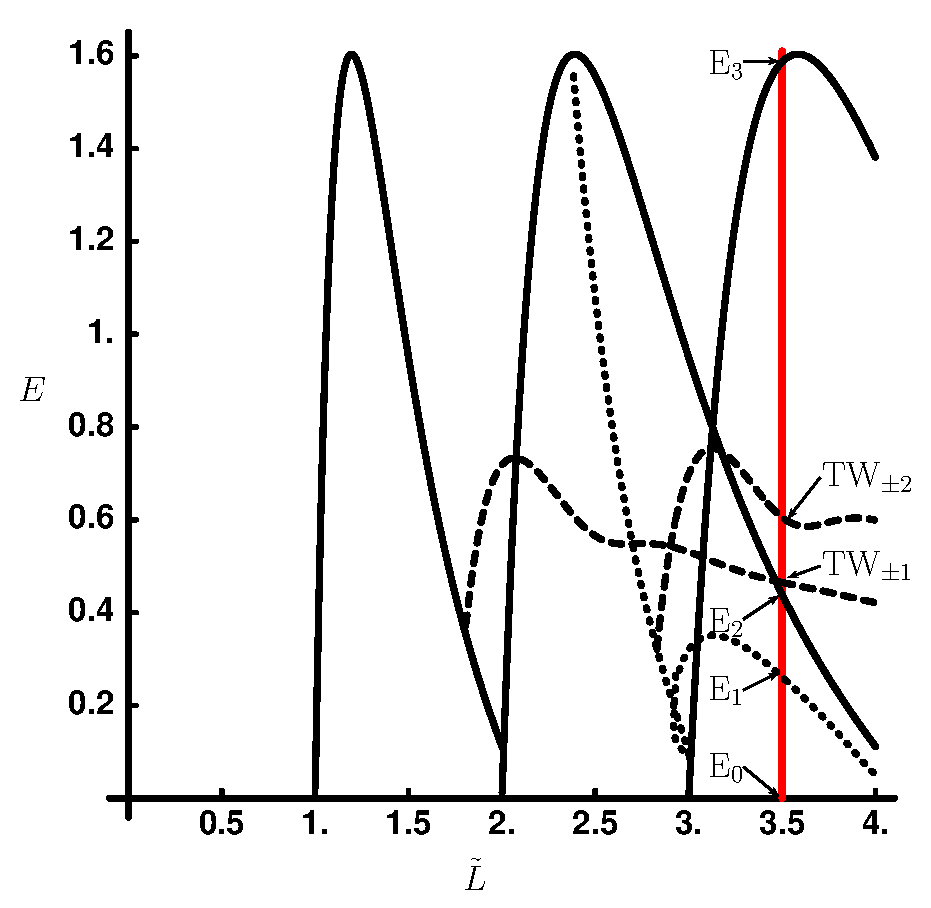
\includegraphics[width=0.5\textwidth]{ksBifDiag_pst}
\end{center}
\caption{\label{fig:SCD07ksBifDiag}
The energy \refeq{SCD07eq:stdks} %{ksEnergy}
of the \eqva\ and \reqva\ that
exist up to $\speriod{}=22$, $\tildeL = 3.5014\ldots$, plotted as a function
of the system size $\tildeL = \speriod{}/2\pi$ (additional \eqva, not present
at $\speriod{} = 22$ are given by Greene and Kim\rf{ksgreene88}). Solid curves denote
$n$-cell solutions \EQV{2} and \EQV{3}, dotted curves the GLMRT
\eqv\ \EQV{1},
and dashed curves the \reqva\ \REQV{\pm}{1} and \REQV{\pm}{2}.
The parameter $\alpha$ of \refrefs{KNSks90,ksgreene88} is
related to the system size by $\tildeL=\sqrt{\alpha/4}$.
(From Cvitanovi{\'c}, Davidchack and Siminos\rf{SCD07})
        }
\end{figure}
%%%%%%%%%%%%%%%%%%%%%%%%%%%%%%%%%%%%%%%%%%%%%%%%%%%%%%%%%%%%%%%%%%

%     BB 2016-02-04, PC 2016-09-23
If $u$ is a temporal \eqv, $u = u(\conf+v\zeit,0)$ whose spatial profile
does not change in time, with a vanishing $u_t=0$ (for an \eqv) or a constant
traveling wave velocity $u_t=v$ (for a \reqv), one can integrate \refeq{e-ks}
\beq
    u_\zeit -v = 0
    = - \left(u^2/2 -u_{\conf}-u_{\conf \conf \conf}\right)_{\conf}
\label{e-ksSteady}
\eeq
once over space, and the highest order derivative in \refeq{e-ksX}
becomes the third order\rf{Mks86,LanThesis,lanCvit07,DoLa14}. We shall
refer to this case as the $\period{}=0$ temporal strip, as specifying $u
= u(\conf_0,0)$ at $\zeit=0$ instant suffices to initialize the spatial
evolution, which in this case is given by a set of three ODEs and an
integration constant, which can be interpreted as the energy density $\expctE$,
\beq
\expctE = {\textstyle\frac{1}{2}}u^2 - c u + u_x + u_{xxx}
\,.
\label{SCD07eq:stdks}
\eeq
% \PCpost{2018-05-30}{
Computationally, it is more robust to compute $\expctE$ by averaging over $\speriod{}$,
as in \refeq{SCD07ksEnergy}.

Eqs.~\refeq{e-ksX}, however, remain a set of four PDEs for any
$\period{}>0$ temporal strip.

\subsubsection{Spatial stability of $u=0$ equilibrium}
\label{sect:KSu0equiS}

To calculate the spatial stability of a spatial \eqv, we need to evaluate
the \stabmat\ of the system in the complex representation \refeq{e-FksX}
in terms of the 16 sub-blocks
\beq
  \Mvar_{ij}^{IJ} (\Fu)  =
\frac{\partial \Fu^{'}{}^{(I)}_i}
     {\partial \Fu{}^{(J)}_j}
\,,\qquad
    \Fu^{'} = \Fu_x
\,.
\ee{eq:StabMatBlocks}
The trivial \eqv\ of \refeq{e-FksX} is given by $\Fu^{(I)}_{j}=0$.
In terms of $[M\!\times\!M]$ temporal Fourier modes blocks its spatial
\stabmat\ is
\beq
\Mvar^{IJ}(0) =
\begin{bmatrix}
  0 & 1 & 0 & 0 \\
  0 & 0 & 1 & 0 \\
  0 & 0 & 0 & 1 \\
\mbox{Diag}\{-i \omega_k\} & 0 & -1 & 0
\end{bmatrix}
\ee{PCeqvaStblty}
%Here
%\beq
%\begin{bmatrix}
%  0 & 1 & 0 & 0 \\
%  0 & 0 & 1 & 0 \\
%  0 & 0 & 0 & 1 \\
%Diag\{-i \omega_k\} & 0 & 0 & 0
%\end{bmatrix}
%\ee{PCcyclic}
%is cyclic of order 4 and thus has a nice characteristic equation, but the
%$\Mvar^{02} (\Fu) =-1$ screws that up.
